\chapter{Регулярные множества и выражения}

В своё время регулярные выражения были прорывом в технике обработки текстов. И они не теряют своих позиций со временем. Регулярные выражения являются частью синтаксиса многих языков программирования\footnote{Например, perl}, в остальных же языках регулярные выражения доступны через функции стандартных библиотек. Более того, так как основным инструментом программиста является текстовый редактор, то практически все достойные внимания среды разработки поддерживают поиск и замену на основе регулярных выражений. Начнем с небольшого теоретического введения. Почерпнуть информацию о регулярных множествах и выражениях можно из \cite{bib:serebryakov:programminglang}.


\section{Формальное определение регулярных множеств и выражений}
Множество --- это фундаментальное, неопределяемое понятие математики. Можно сказать, что множество --- это любая определенная совокупность объектов. Объекты, из которых составлено множество, называются его элементами. Элементы множества различны и отличимы друг от друга. Если $x$ является элементом множества $M$, то говорят что $x$ принадлежит множеству $M$ и сей факт обозначается $x\in M$. В противном случае говорят, что $x$ не принадлежит множеству $M$ и обозначается $x\not\in M$. Если множество небольшое, то его можно задать простым перечислением элементов. Обычно элементы заключают в фигурные скобки и разделяют запятыми. Например, $1\in\{0,1,2\}$, а $3\not\in\{0,1,2\}$. 

Когда множество достаточно велико, то его задают с помощью условия, определяющего принадлежность элемента множеству или задают алгоритм, порождающий элементы множества. Например, множество целых чисел от одного до тысячи можно задать так $\{n|n\text{целое и\ } 1\leq n\leq 1000\}$. Множество не содержащее ни одного элемента, называется пустым и обозначается $\emptyset$. Объединением двух множеств $A$ и $B$ (обозначается $A\cup B$) называется множество, содержащее элементы обоих множеств: $A\cup B=\{x|x\in A\lor x\in B\}$, где $\lor$ - соответствует союзу <<или>>. Например, $\{1,2,3\}\cup\{2,3,4\}=\{1,2,3,4\}$. Результат объединения нескольких множеств $M_0,\ldots,M_n$ записывается так:
\[\bigcup_{i=0}^{n}M_i.\]

Далее мы будем иметь дело с цепочками символов (словами) в алфавите $T$. Цепочкой будем называть упорядоченную последовательность символов. Префиксом, началом или приставкой слова $\omega$ называется цепочка $\omega_1$, если $\omega=\omega_1\omega_2$, а постфиксом или окончанием называется, соответственно, цепочка $\omega_2$. Пустая цепочка, которую далее будем обозначать $\varepsilon$, это такая цепочка, что для любой цепочки $\omega$ справедливо $\omega=\varepsilon\omega=\omega\varepsilon$.

Уже почти все готово, чтобы дать определение \emph{регулярного множества}, а затем и \emph{выражения}, но прежде приведем еще ряд специфичных обозначений. Конкатенацией множеств $A$ и $B$, содержащих цепочки, будет множество $\{\omega_A \omega_B |\omega_A\in A\land \omega_B\in B\}$, где $\lor$ соответствует связке (союзу) <<и>>. Например, конкатенацией множеств $\{a,b,c\}$ и $\{1,2\}$ будет множество из шести элементов $\{a1,a2,b1,b2,c1,c2\}$. Возведением в степень $n$ ($n>0$) множества $A$, обозначаемое как $A^n$, будем называть конкатенацию $AA^{(n-1)}$, причем $A^0=\{\varepsilon\}$. Например,
\[
\{0,1\}^3=\{000,001,010,011,100,101,110,111\}.
\]

Регулярное множество в алфавите символов $T$ рекурсивно определяются так.
\begin{enumerate}
	\item $\emptyset$ --- пустое множество является \emph{регулярным множеством} в алфавите символов $T$.
	\item $\{\varepsilon\}$ --- множество, содержащее пустую цепочку, является \emph{регулярным множеством} в $T$.
	\item $\{s\}$ --- множество, содержащее один символ алфавита ($s\in T$), является регулярным множеством в $T$.
	\item Если $A$ и $B$ --- регулярные множества в алфавите $T$, то регулярными в $T$ также являются множества.
    \begin{enumerate}
        \item $A\cup B$. Объединение множеств.
        \item $AB$. Конкатенация множеств.
    \end{enumerate}
	\item Если $A$ --- регулярное множество в $T$, то итерация 
    \[A^*=\bigcup_{i=0}^{\infty}A^i\] является регулярным множеством в $T$.
	Ничто другое не является регулярным множеством в алфавите $T$.
\end{enumerate}

Отдельного упоминания заслуживает итерация множества $A$ --- бесконечное множество $A^*$, являющееся объединением всех степеней (вплоть до бесконечности) регулярного множества $A$. Например, итерацией множества $\{1\}$ является множество $\{1\}^*=\{\varepsilon,1,11,111,1111,\ldots\}$.

Регулярные множества имеют массу применений на практике. Например, записи чисел, адресов электронной почты (e-mail), URL, имен переменных и констант в языках программирования, и т.д. являются элементами регулярных множеств.

\emph{Регулярное множество} можно задать с помощью \emph{регулярного выражения}. Регулярное выражение в алфавите $T$ и обозначаемое им множество рекурсивно определяются так:

\begin{enumerate}
	\item $\emptyset$ --- регулярное выражение, обозначающее регулярное множество $\emptyset$.
	\item $\varepsilon$ --- регулярное выражение, обозначающее регулярное множество $\{\varepsilon\}$.
	\item $s$ --- регулярное выражение ($s\in T$), обозначающее регулярное множество $\{s\}$.
	\item Если $a$ и $b$ --- регулярные выражения, обозначающие соответственно множества $A$ и $B$ то.
    \begin{enumerate}
        \item $(a|b)$ --- регулярное выражение, обозначающее регулярное множество $A\cup B$. Объединение.
        \item $(ab)$ --- регулярное выражение, обозначающее регулярное множество $AB$. Конкатенация.
    \end{enumerate}

	\item Если $a$ --- регулярное выражение, обозначающее регулярное множество $A$ то, ($a^*$) --- регулярное выражение, обозначающее регулярное множество $A^*$. Итерация.
    \item Ничто другое не является регулярным выражением в алфавите $T$.
\end{enumerate}

Операция итерации имеет наивысший приоритет, затем идет операция конкатенации, затем --- объединения. Поэтому, как и в арифметике, лишние скобки порой (на усмотрение) не пишут: $a|abc^*=(a|((ab)(c^*)))$. Очень часто вместо $aa^*$ пишут $a^+$.

Например, выражение $a(b|c|d)|1$ порождает регулярное множество $\{1,ab,ac,ad\}$. Регулярное выражение $0(0|1|2|3|4|5|6|7)^*$ определяет представление восьмеричных чисел в языке программирования java.


\section*{Задания}
\addcontentsline{toc}{section}{Задания}

\begin{enumerate}
    \item Какое множество порождает регулярное выражение ($\varepsilon$ --- пустая цепочка):
    \begin{enumerate}
        \item $(a|b|\varepsilon)c(d|e)$;
        \item $ac|bd|d(ef|g)$;
        \item $(a|c)d|a(d|\varepsilon)$;
        \item $(0|1)^+(b|\varepsilon)$;
        \item $a|(0|1|2)(b|c)$;
        \item $\varepsilon|(a|\varepsilon)(b|c|d)|\varepsilon$;
        \item $(n|0|p)\varepsilon^*(n|0|p)$.
    \end{enumerate}
    
    \item Опиcать данное множество, используя регулярное выражение.
    \begin{enumerate}
        \item $\{ab1,abc,ab\}$.
        \item $\{ab, c, abab, abc, cab, cc, ababab, ababc,\ldots\}$.
        \item $\{1,01,001,0001,\ldots\}$.
        \item $\{n|\text{$n$ --- четное число в двоичном представлении}\}$.
        \item $\{n|\text{$n$ --- четное число в десятичном представлении}\}$.
        \item $\{s|s=f(k)\land k\in\mathbb{N}\}$, где
        \[f(k)=
            \begin{cases}
                f(0)=a,\\
                f(1)=b,\\
                f(n)=f(n-1)a,n\in\mathbb{N},n>1,n\text{--- четное},\\
                f(n)=f(n-1)b,n\in\mathbb{N},n>1,n\text{--- нечетное}.
            \end{cases}
        \]
        \item $\{\varepsilon,0,1,00,01,11,000,001,011,111,0000,0001,0011,0111,1111,\ldots\}$.
    \end{enumerate}    
\end{enumerate}



\section{FYI:использование регулярных выражений на практике. PCRE}

Так в теории формальных языков формально определяются регулярные выражения. Па практике же, с целью упростить процесс описания регулярных множеств, используют некоторые расширения формально определенных регулярных выражений. Такими расширениями являются, например, регулярные выражения POSIX (Portable Operating System Interface for Unix\footnote{Переносимый интерфейс операционных систем Unix}) или PCRE (Perl Compatible Regular Expressions\footnote{Регулярные выражения, совместимые с используемыми в языке программирования Perl}). 

Мы рассмотрим основные элементы PCRE, ставшие основой практически для всех спецификаций языков программирования и библиотек. Итак, в составе PCRE выделяют:
\begin{itemize}
    \item одиночные символы; 
    \item классы символов; 
    \item альтернативы; 
    \item квантификаторы; 
    \item мнимые символы; 
    \item ссылки на найденный текст;
    \item и т.д.
\end{itemize}

Любой одиночный символ $s$ в составе PCRE соответствует сам себе, если только он не является служебным символом (спецсимволом), играющим особую роль. Служебными символами являются <<\textbackslash>>, <<|>>, <<(>>, <<)>>, <<[>>, <<]>>, <<\{>>, <<\}>>, <<*>>, <<+>>, <<\^{}>>, <<\$>>, <<?>> и <<.>>. Роль этих символов станет ясна в дальнейшем, сейчас же отметим, что если необходимо, чтобы служебный символ соответствовал самому себе, то перед ним нужно поставить символ <<\textbackslash>>. То есть регулярное выражение, производящее поиск символа <<\textbackslash>> в тексте будет выглядеть так <<\textbackslash\textbackslash>>. Кроме того, в PCRE вводятся ряд специальных обозначений, соответствующих нескольким символам или символам, ввод которых затруднен с клавиатуры. Например:

\begin{itemize}
    \item <<\textbackslash d>> – соответствует одной десятичной цифре;
    \item <<\textbackslash D>> – соответствует любому символу, кроме десятичной цифры;
    \item <<\textbackslash s>> – соответствует любому из символов-разделителей (пробельных символов) слов (пробел, табуляция, перевод строки и т.д.);
    \item <<\textbackslash S>> – соответствует любому символу, за исключением пробельного;
    \item <<\textbackslash w>> – соответствует алфавитно-цифровому символу (любой латинской букве, десятичной цифре и знаку подчеркивания <<\_>>) ;
    \item <<\textbackslash W>> – соответствует любому символу, за исключением алфавитно-цифрового;
    \item <<\textbackslash r>>  – символ перевода каретки <CR>;
    \item <<\textbackslash n>>  – символ новой строки <LF>;
    \item <<\textbackslash R>>  – не зависимый от платформы (операционной системы) символ-разделитель строк;
    \item <<\textbackslash xHH>> – соответствие символу ASCII с кодом из двух шестнадцатеричных (HH) цифр;
    \item <<\textbackslash uHHHH>> – соответствие символу Unicode с кодом из четырех шестнадцатеричных (HHHH) цифр.
\end{itemize}

Кроме того, спецсимвол точка <<.>> соответствует любому символу, за исключением символа-разделителя строк.

\emph{Классы символов} определяют соответствие одному символу из множества. Класс --- это список символов, заключенный в квадратные скобки (<<[>>, <<]>> --- спецсимволы). Причем можно указать как отельные символы, так и диапазон. Диапазон задается двумя крайними символами диапазона, разделенными тире. Если требуется указать тире, то перед ним ставится символ <<\textbackslash>>. Например <<[abcde]>> --- любая из букв <<а>>, <<b>>, <<c>>, <<d>>, <<e>>. Это же выражение можно записать короче, так как символы идут по алфавиту: <<[a-e]>>. Если нужно, например, определить класс из знака <<->> и всех цифр, то можно это сделать так: <<[\textbackslash-0123456789]>>, <<[\textbackslash-0-9]>> или, например, <<[\textbackslash-\textbackslash d]>>. Если сразу после открывающей квадратной скобки следует спецсимвол <<\^{}>>, то будет выполняться поиск соответствия символу, не входящему в класс, то есть смысл выражения меняется на противоположный: например, <<[\^{}a-e]>> --- любой символ, \emph{кроме}: <<а>>, <<b>>, <<c>>, <<d>>, <<e>>.

\emph{Альтернативы} --- соответствуют операции объединения в формальном определении регулярных выражений. Альтернативные регулярные выражения разделяются спецсимволом <<|>> и обычно заключаются в круглые скобки. Например, регулярному выражению <<(саша|паша)\textbackslash+(маша|даша)=Л>> соответствует множество из четырех возможных вариантов резьбы по дереву.

\emph{Квантификаторы} ставятся после регулярного выражения и определяют количество повторений шаблона. Выделяют следующие квантификаторы:
\begin{itemize}
    \item <<*>> --- ноль или несколько повторов (итерация в формальном определении);
    \item <<+>> --- один или несколько повторов;
    \item <<?>> --- ноль или один повтор;
    \item <<\{$n$\}>> --- ровно $n$ повторов (здесь $n$ --- натуральное число);
    \item <<\{$n$,\}>> --- по крайней мере $n$ повторов (здесь $n$ --- натуральное число);
    \item <<\{$n$,$m$\}>> --- от $n$ до $m$ повторов (здесь $n,m$ --- натуральные числа).
\end{itemize}

Про <<+>> и <<*>> все известно из формального определения. Остальное лишь более удобная запись:
\[\underbrace{a\cdots a}_n=a\{n\},\]
\[\underbrace{a\cdots a}_na^*=a\{n,\},\]
\[
    \left(
        \underbrace{a\cdots a}_n|
        \underbrace{a\cdots a}_{n+1}|
        \ldots|
        \underbrace{a\cdots a}_{m}|        
    \right)=a\{n,m\},
\]

Отдельно стоит сказать, что по умолчанию квантификаторы <<*>>, <<+>>, <<?>>, <\{$n$,\}>>, <<\{$n$,$m$\}>> являются <<жадными>> (greedy). То есть они выделят по возможности самый длинный фрагмент из всех возможных. Например, при поиске в тексте <<aaaaaaaaaa>> шаблону <<a*a>> будет соответствовать весь текст. Сделать квантификаторы <<ленивыми>> (lazy) можно, поставив после них знак вопроса <<?>>. Тогда в приведенном примере для <<ленивого>> варианта <<a*?a>> результатом поиска будет одна буква <<a>>.

\emph{Мнимые символы} не соответствуют символам текста! Они соответствуют выполнению определенного условия (assertion), например:
\begin{itemize}
    \item <<\^{}>> --- начало строки текста;
    \item <<\$>> --- конец строки или позиция перед символом начала новой строки, расположенного в конце;
    \item <<\textbackslash b>> --- граница слова;
    \item <<\textbackslash B>> --- отсутствие границы слова.
\end{itemize}

Иногда нужно сослаться на подстроку текста, для которой получено совпадение с некоторой частью регулярного выражения. Это можно сделать! Для этого необходимую часть следует заключить в круглые скобки (что конечно не меняет смысл выражения). Каждому выражению, заключенному в скобки будет соответствовать переменная с определенным номером. Чтобы к ней обратится необходимо перед её номером поставить <<\textbackslash>>. Например, если вы желаете найти целое положительное число, являющееся значением элемента XML, то вы можете задать такое выражение: << <(\textbackslash w+)>\textbackslash d+</\textbackslash 1> >>. В переменной \textbackslash 1 будет содержаться текст, который был найден как соответствующий регулярному выражению <<(\textbackslash w+)>>.

На фрагменты текста после поиска можно сослаться и <<извне>> регулярного выражения. Причем независимо от того, в каком виде вы использовали регулярные выражения: при работе с хорошим текстовым редактором, или в создаваемой программе. Условно можно считать, что после того, как поиск был успешно завершен, <<на выходе>> получается массив, содержащий значения соответствующих переменных. В элементе с индексом 0 содержится текст соответствующий шаблону целиком, в элементе с индексом 1 содержится значение, соответствующее первой части регулярного выражения, в элементе с индексом 2 --- второй части и т.д. Так как части регулярного выражения заключенные в скобки могут быть вложенными, то нумеруются они по открывающим скобкам, слева направо. Мы будем обращаться к значениям элементов массива так: \$$n$, где $n$ --- индекс элемента массива (во многих редакторах обращение происходит именно так). Например, если задано регулярное выражение <<(\textbackslash w(\textbackslash w(\textbackslash w)))((\textbackslash w)(\textbackslash w))>> и текст <<ABCDE>>, то значения переменных будут: \$0=<<ABCDE>>, \$1=<<ABC>>, \$2=<<BC>>, \$3=<<C>>, \$4=<<DE>>, \$5=<<D>>, \$6=<<E>>. С помощью ссылок на фрагменты текста, соответствующего шаблону регулярного выражения очень удобно выполнять самые нетривиальные замены в тексте. Например, переставить байты в 32 битном шестнадцатеричном числе в обратном порядке можно так: заменить текст, соответствующий регулярному выражению <<0x([0-9a-fA-F]\{2\})([0-9a-fA-F]\{2\})([0-9a-fA-F]\{2\})([0-9a-fA-F]\{2\})>> на текст <<0x\$4\$3\$2\$1>>. Число <<0x01ABCDEF>> будет заменено на <<0xEFCDAB01>>.

Например, редактор кроссплатформенной среды разработки Eclipse позволяет программисту использовать всю мощь PCRE в процессе написания программы (см. рис. \ref{fig:eclipseIde}).
\begin{figure}
    \centering
    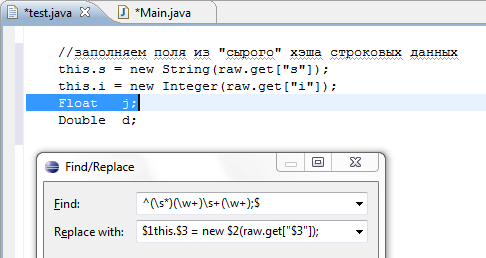
\includegraphics{fig/eclipseIde}
    \caption{Регулярные выражения в IDE Eclipse за работой}\label{fig:eclipseIde}
\end{figure} 

Регулярные выражения позволяют программисту уйти от написания собственных алгоритмов для решения рутинных задач специфичного поиска или замены в тексте, да и обычному пользователю они могут стать неплохим подспорьем при работе с данными в текстовом формате.


\section*{Задания}
\addcontentsline{toc}{section}{Задания}

\begin{enumerate}
    \item Сколько элементов в регулярном множестве, соответствующем регулярному PCRE выражению:
    \begin{enumerate}
        \item <<\textbackslash d\{3,4\}[a-z]\{2\}>>
        \item <<0x[0-9a-fA-F]\{1,8\}>>
        \item <<[0-7]\{1,8\}|(раз|два|три)(четыре|пять)>>
        \item <<\textbackslash d?\textbackslash d?\textbackslash d?>>
        \item <<\^{}\textbackslash b[a-f]\{1,4\}\textbackslash d?\textbackslash b\$>>
        \item <<0[0-7]\{1,7\}?>>
    \end{enumerate}

    \item Организовать в тексте поиск цепочек символов, представляющих собой корректное имя переменной во многих языках программирования: имя начинается с латинской буквы или знака подчеркивания, а заканчивается цепочкой произвольной длины, состоящей из латинских букв, цифр и знака подчеркивания. Имя переменной должно быть отделено от остального текста пустым пространством (пробелом, табуляцией, переносом строки).
    
    \item Организуйте в тексте поиск чисел. Примеры чисел: $0$, $-5$, $0.1$, $-2.24$, $-2.123e-15$, $-31.123E+7$. Запись числа $-31.123E+7$ называется \emph{научной нотацией} и её следует понимать так: $-31.123\cdot 10^{+7}$.
    
    \item Организуйте поиск адресов e-mail в тексте. Примеры адресов: <<kafevm@mail.ru>>, <<e.mail@dot.net.com>>, и т.д.
    
    \item Даты у разных народов пишутся по-разному. Например, в России принято писать сначала день, потом месяц, потом год: <<29.02.1982>>, <<29/02/1982>>. В США, например, даты пишут в таком порядке: месяц, день, год. Выполните замены американских дат российскими, учтя, что разделителями могут быть точка, дефис и косая черта. Числа, соответствующие дням и месяцам не обязательно дополняются ведущим нулем: <<1.1.2011>>. В тексте не встретится сокращенных записей для года (иногда пишут 82 вместо 1982).
    
    \item В базе данных скопилось множество номеров телефонов одного города. Пусть это будет Киров с международным кодом 8(8332). В свое время под номер была отведена строка, и операторы вводили номера телефонов, сообразуясь со своими эстетическими пристрастиями: 8-8332-123456, 8 8332 12 34 56, 8-8332-123-456, 8-8332-12-34-56, 8(8332)12 34 56. И даже без кода: 12 34 56, 123-456. Пора положить конец хаосу. Да будет единый: 8(8332)XX-XX-XX.
    
    \item Некоторая программа принимает на вход табличные данные (товар, цена, количество, ед.изм.) в формате CSV\footnote{}. В процессе их подготовки произошла ошибка и некоторые столбцы поменялись местами: (товар, количество, цена, ед.изм.). Используя регулярные выражения исправьте ошибку.
\begin{verbatim}
товар;   количество;цена;    ед_изм
Молоко;  10;        24.20;   бут.
Кефир;   15;        18.76;   пак.
Печенье; 5;         40.35;   кг.
Хлеб;    20;        24.20;   буханка
Яблоки;  5;         65.30;   кг.
Рельс;   1;         9999.99; шт.
\end{verbatim}
\end{enumerate}
